\cleardoublepage
\chapter{Pré-étude}

%%%%%%%%%%%%%%%%%%%%%%%%%%%%%%%%%%%%%%%%%%%%%%%%%%%%%%%%%%%%%%%%%%%%%%%%%%%%%%%%%%%%%%%%%%
\section{RFID}

Des badges RFID sont mis à disposition des élèves pendant toute la durée de leur formation au sein de l'ETML-ES. Ceux-ci seront utilisés dans ce projet afin d'éviter aux élèves la nécessité de multiples badges.

La technologie du badge a pu être identifiée en utilisant un smartphone (Samsung S23 Ultra) doté de l'application "NFC Tools" (Version 8.9) disponible sur le "Play Store".

La figure \ref{fig:screenshotnfctools} illustre le standard adopté par le badge, en mettant en évidence le fabricant ainsi que le modèle de la puce interne. Des informations techniques plus détaillées sont également disponibles sur le site web du fabricant. \cite{MIFAREClassicEV1}

\begin{figure}[h]
	\centering
	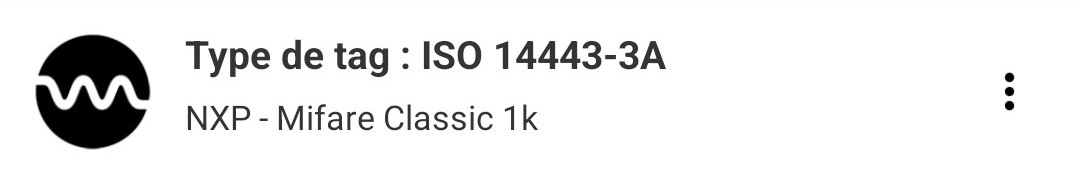
\includegraphics[width=0.7\linewidth]{2312_Images/2312_Pre-etude/Screenshot_NFC_Tools}
	\caption{Type de tag obtenu grâce à "NFC Tools"}
	\label{fig:screenshotnfctools}
\end{figure}

Je me suis alors mis en recherche d'un lecteur RFID. J'ai fait le choix d'un module "tout-en-un" pour faciliter le design, notamment de l'antenne. Deux modules se sont distingués : 

\vspace{5pt}
\href{https://www.mikroe.com/rfid-click}{Module MikroE "RFID CLICK"} : Ce module a été utilisé dans des projets précédents. Il est disponible en quantité suffisante et fait partie des prix les plus bas. Néanmoins, il a le désavantage de devoir être monté sur le PCB en prenant un espace non négligeable. De plus, cela offre peu de flexibilité quant à son placement et augmente le risque que le badge ait des difficultés à être lu une fois le boitier monté. 

\vspace{5pt}
\href{https://www.mikroe.com/rfid-click}{Module Eccel "RFID NFC Chilli UART-B1"} : Ce module offre le principale avantage d'être plus flexible dans son placement. Il est facilement contrôlable par l'UART et toute la documentation sur les commandes à utiliser sont disponibles. 

%%%%%%%%%%%%%%%%%%%%%%%%%%%%%%%%%%%%%%%%%%%%%%%%%%%%%%%%%%%%%%%%%%%%%%%%%%%%%%%%%%%%%%%%%%
\section{Alimentation}
L'entiereté du circuit sera alimenté par 3V3 car le microcontrôleur et le module rfid utilisent tout deux du 3V3. 
Donc j'utilise un module monobloc d'alimentation 230V à 3V3. 

%%%%%%%%%%%%%%%%%%%%%%%%%%%%%%%%%%%%%%%%%%%%%%%%%%%%%%%%%%%%%%%%%%%%%%%%%%%%%%%%%%%%%%%%%%
\section{Ethernet}

%%%%%%%%%%%%%%%%%%%%%%%%%%%%%%%%%%%%%%%%%%%%%%%%%%%%%%%%%%%%%%%%%%%%%%%%%%%%%%%%%%%%%%%%%%
\section{Boitier}
Le boitier sera réalisé en impression 3D. Cette méthode offre l'avantage d'une plus grande flexibilité.
Pour des raisons de sécurité, le plastique utilisé devra être résistant à la chaleur et non sensible à l'humidité. C'est le cas du PLA qui ne peut donc pas être utilisé dans cette application ou il y a de la haute tension.

%%%%%%%%%%%%%%%%%%%%%%%%%%%%%%%%%%%%%%%%%%%%%%%%%%%%%%%%%%%%%%%%%%%%%%%%%%%%%%%%%%%%%%%%%%
\section{Relais}
J'ai du faire le choix d'un relais pour commuter le 230VAC. J'ai choisi un relais capable de supporter un courant suffisamment élevé pour supporter le courant maximal que peut fournir la prise murale. J'ai dû m'assurer que la tension de contrôle soit aussi assez basse pour pouvoir correspondre à l'alimentation de mon circuit.
J'ai fait le choix aussi d'un relai à verrouillage pour permettre de réduire la consommation de courant après la commutation en conservant ainsi son état.

Le relais nécessite d'avoir une diode en série de ses bobines de set et reset (voir datasheet).
De plus, un circuit de protection doit être mis en place. Et il faut des mosfet pour les piloter.

%%%%%%%%%%%%%%%%%%%%%%%%%%%%%%%%%%%%%%%%%%%%%%%%%%%%%%%%%%%%%%%%%%%%%%%%%%%%%%%%%%%%%%%%%%
\section{Connecteurs 230VAC}
Les connecteurs doivent être en mesure de supporter le courant maximal qui puisse être fourni par une prise murale. Ils doivent aussi présenter suffisamment d'isolation pour la tension du réseau.


%%%%%%%%%%%%%%%%%%%%%%%%%%%%%%%%%%%%%%%%%%%%%%%%%%%%%%%%%%%%%%%%%%%%%%%%%%%%%%%%%%%%%%%%%%
\section{Base de donnée}
La base de donnée sera géré par un Raspberry Pi. Cette solution offre la flexibilité d'un ordinateur avec une consommation minime. La gestion sera réalisé en langage Python.
